\documentclass{crypto-exercise}
\usepackage{amsthm}
\author{Sven Laur}
\contributor[Initial solution]{Sanja Scepanovic}
\contributor[Streamlining of arguments]{Sven Laur}
\editor{Sven Laur}
\tags{computational indistinguishability, distributions, hybrid argument}

\renewcommand{\ADVIND}[2]{\ADV^{\mathsf{ind}}_{#1}(#2)}
\newcommand{\ts}{t_{\mathrm{s}}}

\begin{document}
\begin{exercise}{Classical hybrid argument}
Let $\XXX_0$ and $\XXX_1$ efficiently samplable distributions that are $(t, \varepsilon)$-indistinguishable. Show that distributions $\XXX_0$ and $\XXX_1$ remain computationally indistinguishable even if the adversary can get $n$ samples.
As the first step, estimate computational distances between following games
\begin{align*}
  & \begin{game}{\GAME_{00}^\AD}
    &  x_0 \gets \XXX_0 \\
    &  x_1 \gets \XXX_0 \\
    & \RETURN \AD(x_0,x_1)
  \end{game} 
&
 & \begin{game}{\GAME_{01}^\AD}
    &  x_0 \gets \XXX_0 \\
    &  x_1 \gets \XXX_1 \\
    & \RETURN \AD(x_0,x_1)
  \end{game} 
&
 & \begin{game}{\GAME_{11}^\AD}
    &  x_0 \gets \XXX_1 \\
    &  x_1 \gets \XXX_1 \\
    & \RETURN \AD(x_0,x_1)
  \end{game} 
&
\end{align*}
and then generalise the argumentation to the case, where the adversary $\AD$ gets $n$ samples from a distribution $\XXX_i$.  Why do we need to assume that distributions $\XXX_0$ and $\XXX_1$ are efficiently samplable?
\end{exercise}


\begin{solution}
Let us examine computational distances between following games:
\begin{align*}
  & \begin{game}{\GAME_{00}^\AD}
    &  x_0 \gets \XXX_0 \\
    &  x_1 \gets \XXX_0 \\
    & \RETURN \AD(x_0,x_1)
  \end{game} 
&
 & \begin{game}{\GAME_{01}^\AD}
    &  x_0 \gets \XXX_0 \\
    &  x_1 \gets \XXX_1 \\
    & \RETURN \AD(x_0,x_1)\enspace.
  \end{game} 
\end{align*}
Note that we can define the next adversary:
\begin{align*}
  & \begin{game}{\ADB(x)}
    &  x_0 \gets \XXX_0 \\
    &  x_1 \gets x \\
    & \RETURN \AD(x_0,x_1)
      \end{game} 
\end{align*}
against indistinguishability games
\begin{align*}
  & \begin{game}{\BGAME_0^\ADB}
    &  x \gets \XXX_0 \\
    & \RETURN \ADB(x)
  \end{game} 
&
 & \begin{game}{\BGAME_1^\ADB}
   &  x \gets \XXX_1 \\
    & \RETURN \ADB (x)\enspace. 
    \end{game} 
\end{align*}
Inserting our concrete adversary $\ADB$ into the indistinguishability games yields:
\begin{align*}
  & \begin{game}{\BGAME_0^{\ADB}}
    &  x \gets \XXX_0 \\
    &  x_0 \gets \XXX_0 \\
    &  x_1 \gets x \\
    & \RETURN \AD(x_0,x_1)
  \end{game} 
&
 & \begin{game}{\BGAME_1^{\ADB}}
   &  x \gets \XXX_1 \\
    &  x_0 \gets \XXX_0 \\
    &  x_1 \gets x \\
    & \RETURN \AD(x_0,x_1)\enspace,
    \end{game}
\end{align*}
from which we can easily see that games $\BGAME_0^\ADB$ is equivalent to $\GAME_0^\AD$ and $\BGAME_1^\ADB$ is equivalent to $\GAME_1^\AD$ (denoted by $\BGAME_0^\ADB\equiv\GAME_0^\AD$ and $\BGAME_1^\ADB\equiv\GAME_1^\AD$). That leads to the next inequality
\begin{align*}
\abs{\pr{\GAME_{00}^{\AD}] = 1} - \pr{\GAME_{01}^{\AD} = 1}}=\abs{\pr{\BGAME_0^{\ADB}] = 1} - \pr{\BGAME_1^{\ADB} = 1}} \leq \ADVIND{\XXX_0,\XXX_1}{\ADB}\enspace. 
\end{align*}
Let $\ts$ denote the time needed to take a sample form $\XXX_0$ and $t_\AD$ the running time of $\AD$. Then the running time of $\ADB$ is $t_s$ + $t_{\AD}$. Now if if $t_\AD\leq t-\ts$, the running time of $\ADB$ is at most $t$ and we can bound
\begin{align*}
\ADVIND{\XXX_0,\XXX_1}{\ADB}\leq \varepsilon\enspace.
\end{align*} 
More formally, note that $(t,\varepsilon)$-indistinguishability of $\XXX_0$ and $\XXX_1$ implies that this equation must hold for any $t$-time adversary $\ADB$ and thus it must hold for the particular construction of $\ADB$.  

In a similar way, we can analyse the computational distances between the games:
\begin{align*}
  & \begin{game}{\GAME_{01}^\AD}
    &  x_0 \gets \XXX_0 \\
    &  x_1 \gets \XXX_1 \\
    & \RETURN \AD(x_0,x_1)
  \end{game} 
&
 & \begin{game}{\GAME_{11}^\AD}
    &  x_0 \gets \XXX_1 \\
    &  x_1 \gets \XXX_1 \\
    & \RETURN \AD(x_0,x_1)\enspace.
  \end{game} 
\end{align*}
In this case, we obtain reduction to the indistinguishability by considering the following adversary 
\begin{align*}
  & \begin{game}{\ADC(x)}
    &  x_0 \gets x \\
    &  x_1 \gets \XXX_1 \\
    & \RETURN \AD(x_0,x_1)\enspace.
      \end{game} 
\end{align*}
Direct substitution into the games $\BGAME_0$ and $\BGAME_1$ allows us to prove that $\BGAME_0^\ADC\equiv\GAME_0^\AD$ and $\BGAME_1^\ADC\equiv\GAME_1^\AD$.  Thus,
\begin{align*}
\abs{\pr{\GAME_{01}^{\AD}] = 1} - \pr{\GAME_{11}^{\AD} = 1}} =\ADVIND{\XXX_0,\XXX_1}{\ADC}  
\end{align*}
Again, it is easy to see that if we can sample an element from $\XXX_1$ in time $\ts$, then  
\begin{align*}
\abs{\pr{\GAME_{01}^{\AD}] = 1} - \pr{\GAME_{11}^{\AD} = 1}} \leq \varepsilon
\end{align*}
for all $(t-\ts)$-time adversaries $\AD$. Finally, we can use triangular inequality to combine both bounds:
\begin{align*}
\abs{\pr{\GAME_{00}^{\AD}]=1} - \pr{\GAME_{11}^{\AD}=1}}\leq
\abs{\pr{\GAME_{00}^{\AD}]=1} - \pr{\GAME_{01}^{\AD}=1}} +
\abs{\pr{\GAME_{01}^{\AD}]=1} - \pr{\GAME_{11}^{\AD}=1}} \leq 2 \varepsilon\enspace.
\end{align*}
As the bound holds for any $(t-\ts)$-time adversary $\AD$, we have established that game $\GAME_{00}$ and $\GAME_{11}$ are $(t-\ts,2\varepsilon)$-indistinguishable.

\vspace*{2ex}
\noindent
\textsc{Genralisation.}
To generalise the result, we must consider the following set of games
\begin{align*}
  & \begin{game}{\GAME_{b_{n-1}\ldots b_1 b_0}^\AD}
    &  x_0 \gets \XXX_{b_0} \\
    &  x_1 \gets \XXX_{b_1} \\
    & \ldots\\
    &  x_{n-1} \gets \XXX_{b_{n-1}} \\
    & \RETURN \AD(x_0,x_1,\ldots,x_{n-1})\enspace.
  \end{game} 
\end{align*}
It is easy to see that for any two games $\GAME_{b_{n-1}\ldots b_1 b_0}$ and $\GAME_{c_{n-1}\ldots c_1 c_0}$ where indices differ only in the $i^{\text{th}}$ position we can define a reduction adversary $\ADB$ which samples all other elements according to the description of $\GAME_{b_{n-1}\ldots b_1 b_0}$ and uses the sample $x$ in the place of $x_i$. If $b_i=0$ then by the construction $\BGAME_0^\ADB\equiv \GAME_{b_{n-1}\ldots b_1 b_0}^\AD$ and  $\BGAME_1^\ADB\equiv \GAME_{c_{n-1}\ldots c_1 c_0}^\AD$. Otherwise, $\BGAME_0^\ADB\equiv \GAME_{c_{n-1}\ldots c_1 c_0}^\AD$ and $\BGAME_1^\ADB\equiv \GAME_{b_{n-1}\ldots b_1 b_0}^\AD$. As the running time of $\ADB$ is $t_\AD+(n-1)\ts$, we get that for all $(t - (n-1)\ts)$-time adversaries $\AD$:
\begin{align*}
\abs{\pr{\smash{\GAME_{b_{n-1}\ldots b_1 b_0}^\AD=1}}- \pr{\smash{\GAME_{c_{n-1}\ldots c_1 c_0}^\AD=1}}}\leq \varepsilon.
\end{align*}
  
To bound the computational distance between $\GAME_{0\ldots0}$ and $\GAME_{1\ldots1}$, we have to find a path from $0\ldots0$ to $1\ldots1$ where adjacent points in the path differ only by single bit. The longest such paths goes through all $2^n$ bitstrings while the simplest one has only $n$ alterations. Since each edge in this path adds $\varepsilon$ to the estimate on the computational distance, we should use the shortest path. As a consequence, we can prove that games  
$\GAME_{0\ldots0}$ and $\GAME_{1\ldots1}$ are $(t-(n-1)\ts,n\varepsilon)$-indistinguishable. Figure~\ref{fig:hyper-cube} illustrates the derivation when $n=3$.   

\begin{figure}[H]
\begin{center}
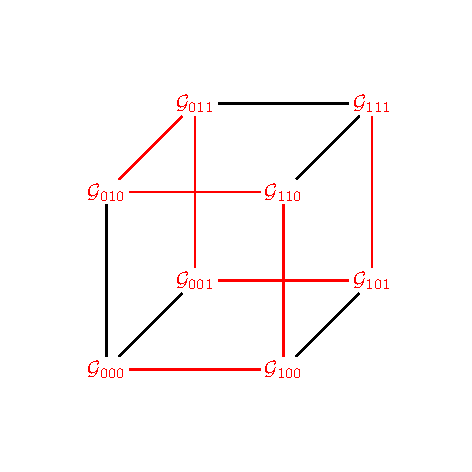
\includegraphics[scale=0.8]{./figures/0306-hypercube-i}
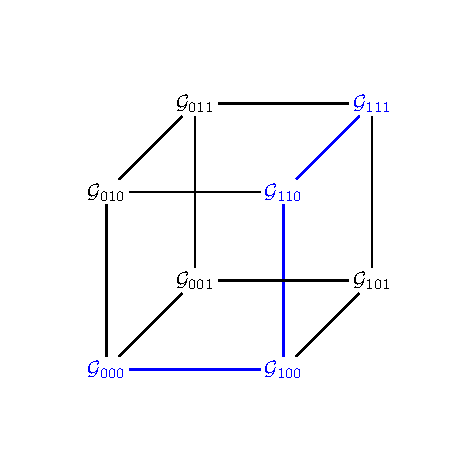
\includegraphics[scale=0.8]{./figures/0306-hypercube-ii}
\end{center}
\caption{Game space when the number of samples is three with the longest and the shortest path}
\label{fig:hyper-cube}
\end{figure}


\end{solution}
\end{document}